%%
%% Beuth Hochschule für Technik 
%%
%% Einleitung 1
%%
%%

\newpage
[Hansert]
\section{Zu regelndes Objekt kennen lernen}
Bei dem zu regelnden Objekt handelt es sich um einen elektrischen, steuerbaren, hydraulischen Druckgenerator für den Antrieb einer Arbeitsmaschine. Zu beachten ist, das es sich um eine simulierte Druckregelstrecke handelt. Bekannte Größen sind:

\begin{itemize}
\item Steuerspannung -10V $\leq u(t) \leq$ 10V, wobei nur der positive Bereich betrachtet wird, da der Druck von 0 bis zu einem Maximalwert verstellt wird

\item die Messgröße $Y_{M}(t)$ wird in Form einer Spannung gemessen

\item der Verstärkungsfaktor der Messeinrichtung $V_{M}$ beträgt $0,08\frac{V}{Bar}$

\item bei einer Grundlast liegt der Arbeitspunktdruck bei $50Bar$

\item die Messeinrichtung hat ein PT1-Verhalten, bei welchem die Zeitkonstante vernachlässigt werden kann 
\end{itemize}


Wenn man das Objekt (Abbildung \ref{RegelKreis}) genauer betrachtet, können die Teile eines Standard-Regelkreises erkannt werden:
\begin{itemize}
\item $u(t)$ Regelgröße
\item $y(t)$ Stellgröße
\item Stelleinrichtung und Regelstrecke
\end{itemize}

\begin{figure}[htbp]
	\begin{center}
		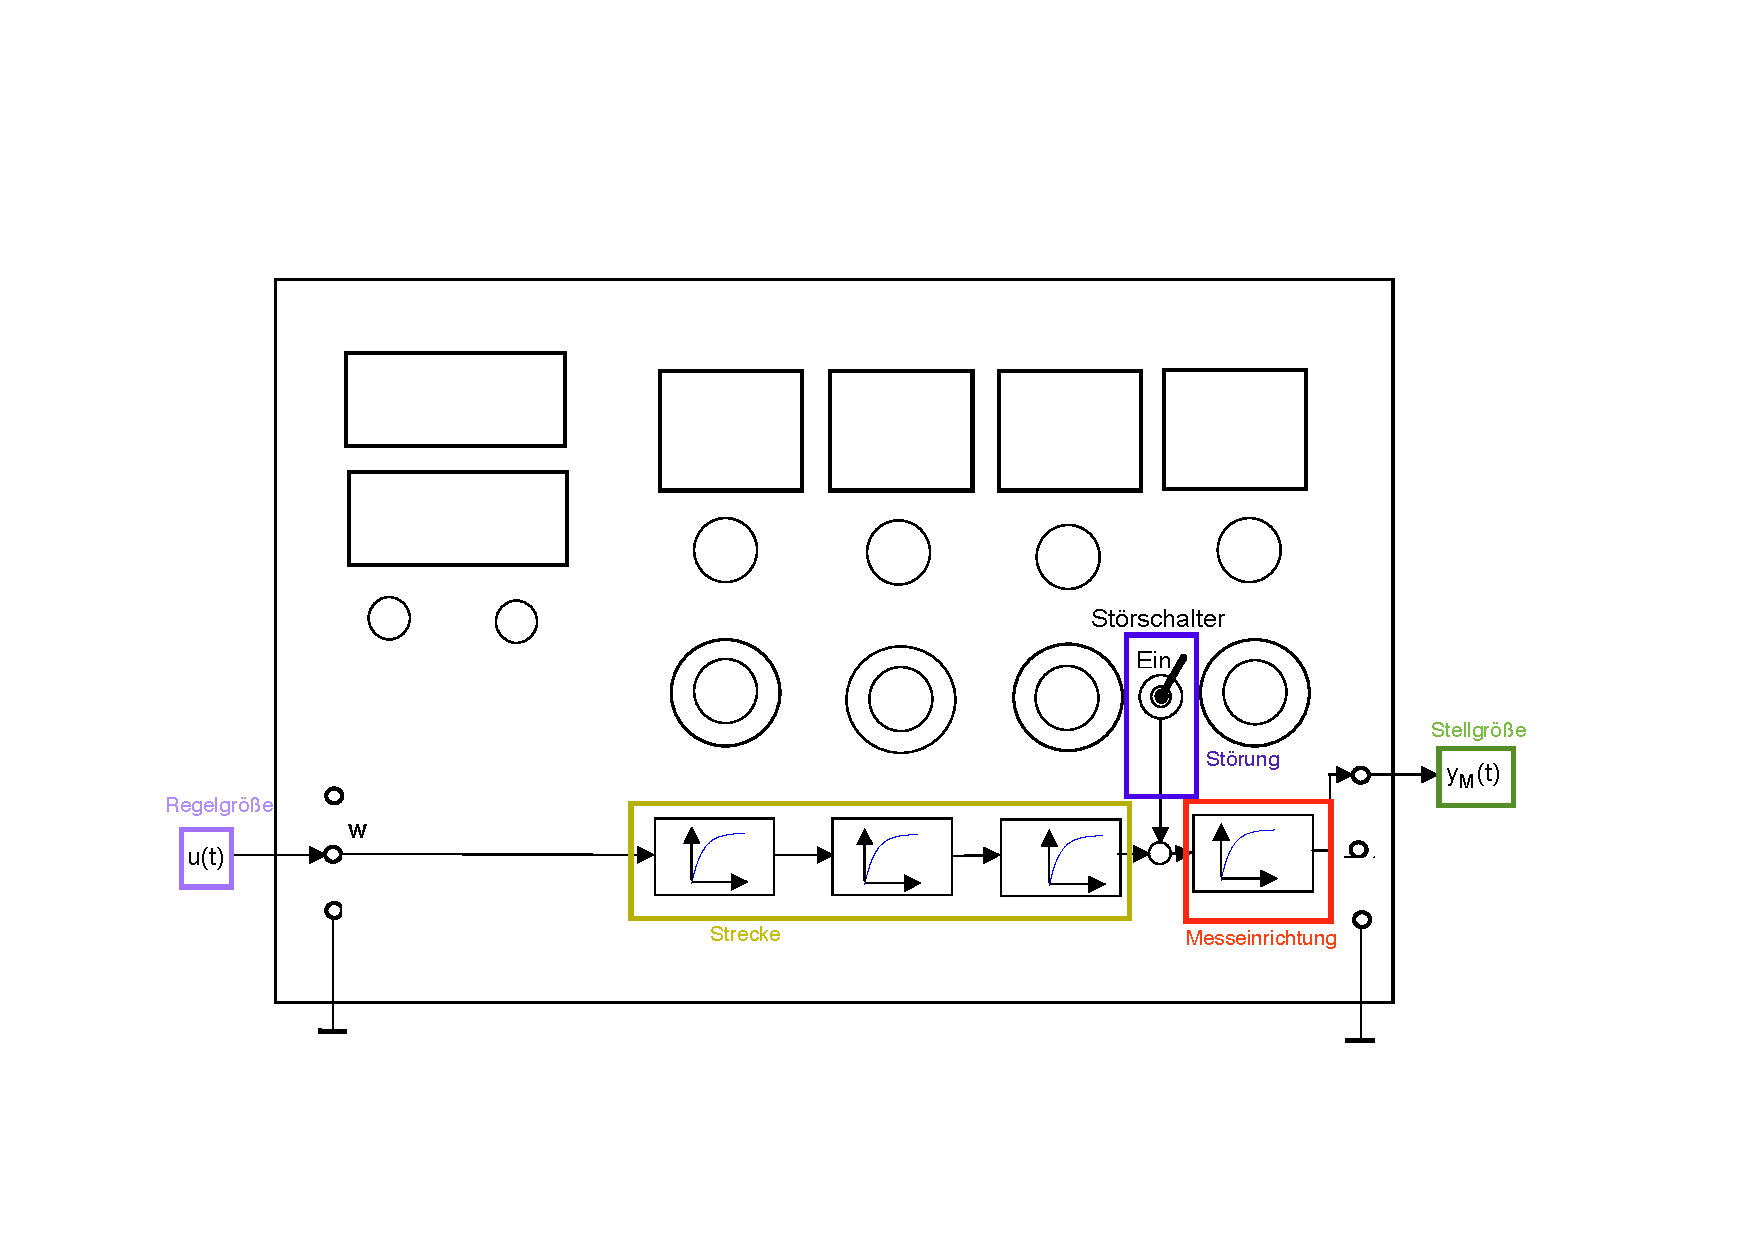
\includegraphics[scale=0.4]{regelkreis.pdf}
		\caption{Elektrische simulierte Druckregelstrecke mit Standard-Regelkreis}
       \label{RegelKreis}
	\end{center} 
\end{figure}

\newpage

Um alle Größen zu bestimmen bzw. zu messen und um den Reger zu entwickeln, werden die Programme MATLAB/Simulink eingesetzt. Dies geschieht mit dem Tool Real-Time-Workshop und einer A/D-D/A Wandlerkarte.


\subsection{Offset}
Um das System mit dem Rechner zu verbinden wird eine Wandlerkarte eingesetzt. Die Wandlerkarte ist im PC eingebaut. Um Fälschungen im Ergebnis zu umgehen, muss der Eingangs- und Ausgangsoffset gemessen werden. Um diese Werte zu messen wurde das \textit{reinraus2007b.mdl} Simulinkmodell benutzt.\\

Für den Eingangsoffset der Wandlerkarte wurde ein Display für die Ausgabe benutzt. Wichtig ist, dass die Leitungen für die Verbindung von der Wandlerkarte zum System kurzgeschlossen werden. Auf dieser Weise werden zum Beispiel $5V$ angelegt und diese $5V$ werden vom Ergebnis subtrahiert. Unser Eingangsoffset beträgt $0,1292V$.\\

Um den Ausgangsoffset zu ermitteln werden die zwei Leitungen an ein Voltmeter angeschlossen. Dieser sollte bei einem nicht vorhandenen Offset null zeigen. In unserem Fall konnten wir einen Ausgangsoffset von $0,1050V$ ablesen.\\

Diese beide Werte werden bei Simulationen in den Kapiteln \ref{Kapitel5} und \ref{Kapitel7} jeweils  subtrahiert, um die Verfälschung von Ergebnissen zu vermeiden.


%%%%%%%%%%%%%%%%%%%%%%%%%%
%% bild einfügen

%\begin{figure}[h]
%	\begin{center}
%		\includegraphics[scale=0.5]{pic.jpg}
%		\caption{bildbeschreibung - titel}
%       \label{für referenzen}
%	\end{center} 
%\end{figure}